\documentclass[12pt]{standalone}
\usepackage{tikz}


\begin{document}
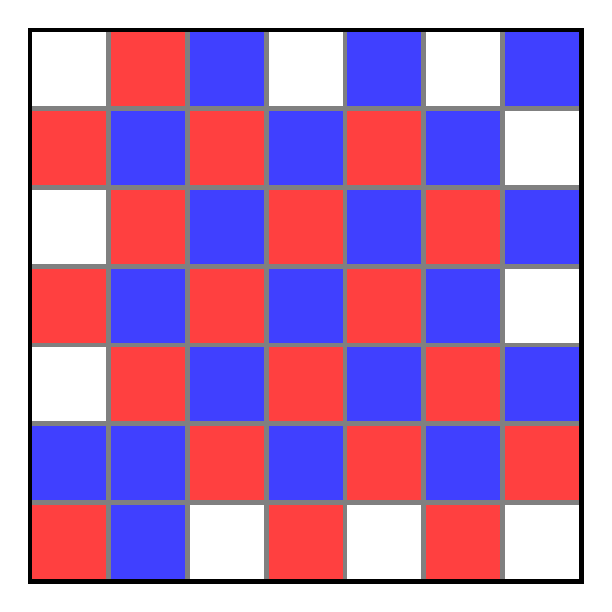
\begin{tikzpicture}
    \fill[red!75]\foreach \a in
        {(0,0), (3,0), (5,0), (2,1), (4,1), (6,1), (1,2), (3,2), (5,2), (0,3), (2,3), (4,3), (1,4), (3,4), (5,4), (0,5), (2,5), (4,5), (1,6)} {\a rectangle +(1,1)};
    \fill[blue!75]\foreach \a in 
        {(1,0), (0,1), (1,1), (3,1), (5,1), (2,2), (4,2), (6,2), (1,3), (3,3), (5,3), (2,4), (4,4), (6,4), (1,5), (3,5), (5,5), (2,6), (4,6), (6,6)} {\a rectangle +(1,1)};
    \draw[black!50, line width=0.6mm] (0,0) grid (7,7);
    \draw[black, line width=0.6mm] (0,0) rectangle (7,7);
\end{tikzpicture}
\end{document}
% FSI_7x7_DS